    \chapter{Especificação técnica} \label{cap:especificacao_tecnica}

\section{Análise de Contexto}

    \subsection{Visão Geral}
    O desenvolvimento deste protótipo tem a finalidade de auxiliar o professor no ensino de programação para crianças.
    
    O software, apresentado em forma de jogo com o tema reciclagem, apresentará diversos desafios em que a criança deverá solucionar criando sequências lógicas com blocos físicos. Após a ordenação dos blocos, de maneira em que achar correta, pela criança, ela deverá tirar fotos da sua solução e submetê-la para a avaliação do desafio dentro do aplicativo.
    
    Ao finalizar a captura da solução proposta, o aplicativo enviará a sequência de imagens para um servidor, hospedado na nuvem, o qual fará a análise das imagens dos blocos
    por meio de visão computacional a fim de identificar e converter os blocos em ações para o jogo.
    
    Ao final da conversão, o servidor devolverá para o jogo a solução proposta em ações.
    Caso a solução esteja correta, a criança passará para o próximo desafio, caso contrário, será oferecido uma nova tentativa.
    
    O aplicativo coletará dados durante o desafio para o preenchimento de relatórios que serão apresentados para o professor ou tutor através de um portal.
    
    A figura \ref{figura:diagrama_blocos} apresenta a visão geral do sistema proposto.
    
    \begin{figure}[h!]
        \centering
        \caption{Visão geral do sistema}
        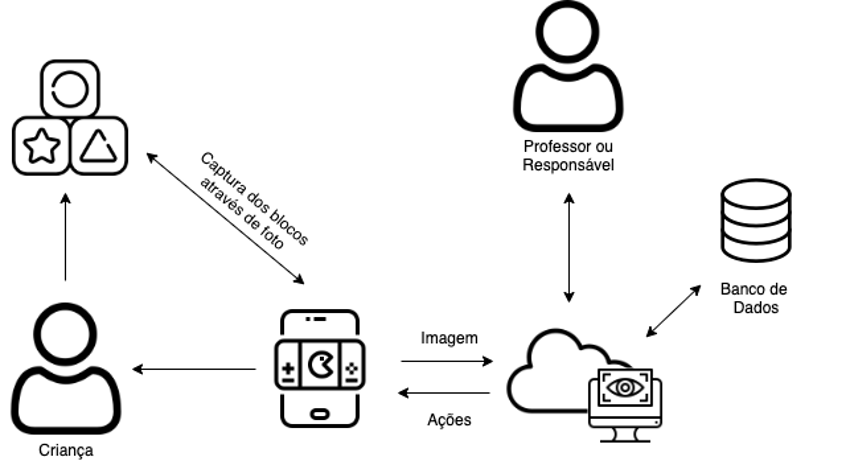
\includegraphics[width=12cm]{images/cap3/diagrama_blocos.png}
        \caption*{Fonte:o autor (2020)}
        \label{figura:diagrama_blocos}
    \end{figure}
    
    \subsection{Condições Restritivas}
    O projeto proposto apresenta algumas condições restritivas, conforme descrito
    nos próximos subitens.

        \subsubsection{Custos}
        Apesar do aplicativo jogo precisar de materiais relativamente baratos para funcionar, como blocos impressos em 3D ou até mesmo papéis coloridos dobrados de formas semelhante aos blocos impressos, ainda se faz necessário o uso de um celular com sistema operacional andoird com câmera para que o aplicativo funcione. 
        
        \subsubsection{Físicas e Ambientais}
        
        \subsubsection{Tecnológicas}
        O aplicativo jogo necessita de um celular com câmera e com o sistema operacional Android com a versão igual ou superior a 5.0- Lollipop. Por se tratar de um protótipo, o aplicativo jogo não oferece suporte para os demais dispositivos móveis com outros sistemas operacionais como por exemplo Iphones. 
        
        \subsubsection{Energização}
        O celular é limitado em relação à energia, tendo um período máximo que uma carga pode sustentar, esse período máximo varia conforme o modelo e o uso do dispositivo. Para diminuir os efeitos causado por essa limitação, recomenda-se o uso do aplicativo com a bateria cheia ou próximo a uma tomada caso seja necessário recarregar a bateria do dispositivo móvel.   
        
        \subsubsection{Interferências devido ao meio}
    
     \subsection{Benefícios e Impactos}
    O aplicativo jogo apresenta alguns benefícios e impactos, conforme descrito nos próximos subitens.

        \subsubsection{Econômicos}
        Além de um celular com câmera, o aplicativo jogo proposto é capaz de funcionar com recursos relativamente baratos, como blocos impressos em 3D ou até mesmo uma folha colorida dobrada em formatos semelhantes aos cubos; o aplicativo jogo também funciona de forma simples. Portanto pode ser utilizado em casa ou implantado em escolas de forma fácil e econômica para proporcionar a crianças um contato inicial com temas como lógica de programação e sustentabilidade, além de atender às novas demandas da BNCC para o ensino.
        
        \subsubsection{Operacionais}
        
        \subsubsection{Estratégicos}
        
        \subsubsection{Políticos}
        A mais nova atualização da Base Nacional Comum Curricular destina uma de suas dez competência a educação integral por meio de tecnologias digitais e faz uso, no caderno de matemática, do termo “pensamento computacional”. Pensando nisso, o aplicativo jogo proposto possibilita, de uma forma simples e econômica, um meio para trabalhar essas competências nas escolas. 

        \subsubsection{Sociais}
        O aplicativo jogo apresenta benefícios sociais para as crianças, pois as crianças terão acessos a conceitos básicos de lógica de programação e oportunidade de exercitar esse conceitos, o que pode auxiliar em competências como raciocínio lógico, resolução de problemas, pensamento computacional, entre outras habilidades que tem sido cada vez mais requisitadas no mercado de trabalho. Isso sendo proporcionado por um jogo, além de gerar maior engajamento no ensino de crianças, pode desenvolver  também competências como cooperação, cumprimento de regras, controle de impulsividade, auxílio na tomada de decisões, mais facilidade para lidar com erros e fracassos entre outras habilidades sociais.
        Além disso, o aplicativo jogo, por meio do tema de reciclagem, pode desenvolver senso de sustentabilidade auxiliando na compreensão da importância do descarte correto do lixo, o que impacta direta e positivamente  o meio ambiente.

\section{Análise Funcional e de Requisitos Tecnológicos}

    \subsection{Lista de Funcionalidade e Atores}
    O sistema será composto  pelas seguintes funcionalidades:
    \begin{itemize}
        \item Desafios de lógica com o tema reciclagem;
        \item Identificação dos blocos;
        \item Conversão dos blocos em ações;
        \item Relatórios de jogo para acompanhamento do professor;
    \end{itemize}
    
    O sistema tem como atores a criança e professor/tutor.
    
    A criança é responsável pela interação com os blocos e aplicativo.
    O professor/tutor é responsável pela interação com os dados adquiridos durante a partida da criança.
    
    \subsection{Comunicação}
    A comunicação entre o aplicativo e o servidor ocorrerá de maneira unidirecional e utilizará arquitetura \textit{REST}, através da conexão Wi-Fi com a Internet.
    A comunicação entre o aplicativo e o servidor ocorre de maneira unidirecional. 
    O aplicativo envia os dados e imagens para o servidor. Após o servidor salvar os dados e processar as imagens, ele retorna para o aplicativo.
    
    \subsubsection{REST}
    O \textit{REST (Representational State Transfer)} é uma abstração da arquitetura da \textit{Web}. Consistem em regras que permitem a criação de projetos com interfaces bem definidas, permitindo a comunicação entre aplicações.
    
    
%     \subsection{Processamento}
    
%     \subsection{Interface Homem-Máquina}
    
%     \subsection{Sistemas Controlados Automaticamente}
    
%     \subsection{Aquisição de dados e Atuação}


\section{Análise da Arquitetura do Sistema}

    \subsection{Hardware}
    O hardware do sistema será composto por blocos físicos e o dispositivo mobile com câmera.
    
    Os blocos físicos serão construídos de PLA, impressos em 3D, com o tamanho aproximado de 10cm x 10cm x 5cm, seus cantos serão arredondados para evitar acidentes no manuseio. Para facilitar a identificação, além da sua cor, cada bloco possuirá um simbolo representado o tipo da ação.
    
    O dispositivo mobile deverá ser um celular \textit{Android} com camêra, podendo variar entre os modelos existentes no mercado.
    
    % \subsection{Software}

